% !TeX spellcheck = en_US
\documentclass[final,hyperref={pdfpagelabels=false}]{beamer} 

\mode<presentation> {  
  \usetheme{UOSSYSPoster}    
}

\usepackage[english]{babel}
\usepackage[utf8]{inputenc}
\usepackage{amsmath,amsthm, amssymb, latexsym}
\usepackage{svg}
\usepackage{epsfig}
\usepackage{multirow}
\usepackage{pifont}
\usepackage{algpseudocode}
\usepackage{colortbl}
\usepackage{booktabs}
\usepackage{lipsum} 
\usepackage{tikz}
\usepackage{qrcode}
\usepackage{booktabs}




\usefonttheme[onlymath]{serif}

\boldmath
\usepackage[orientation=portrait,size=a0,scale=1.5,debug]{beamerposter}                       

\morelogos{\hspace{1cm}\qquad\qquad\includesvg[height=4cm]{logos/rso_logo}}



\title{Assessing the suitability of different sensor types for deriving soil related differences in plant characteristics}
\author{Maren Pöttker¹, Manuel Reese¹, Thomas Hänel², Thomas Jarmer¹ \\\,\\ \footnotesize{\textit{¹Remote Sensing Group,  Institute of Computer Science, Osnabrück University, 49090 Osnabrück, Germany, maren.poettker@uos.de, manresse@uos.de, thomas.jarmer@uos.de\\²Distributed Systems Group, Institute of Computer Science, Osnabrück University, 49090 Osnabrück, Germany, haenel@uos.de}}}
\footerline{}

\begin{document}
\begin{frame}
\centering

\begin{minipage}[t][20cm][t]{0.315\paperwidth}


\begin{block}{Introduction}
\centering
\begin{minipage}{0.95\textwidth}
\small{\begin{itemize}
    \item Different soil types provide nutrients and water to crops in varying quantities \cite{saxton1986estimating}
    \item Knowledge about spatial variability in soils is crucial for site-specific management and precision agriculture \cite{khosla2002use}
    \item Remote sensing data can be used to derive soil related differences in plants from its spectral information \cite{weiss2020remote}
    \item Goal: Comparison of three optical sensor systems for soil related plant characteristics
\end{itemize}}
\vspace{0.65cm}
\end{minipage}
\end{block}
\end{minipage}
\hspace{4mm}
\begin{minipage}[t][20cm][t]{0.315\paperwidth}
\begin{block}{Sensor Systems }
\begin{minipage}{0.95\textwidth}
\centering
\end{minipage}
\vspace{0.3cm}
\begin{minipage}{0.95\textwidth}
\small{
Three multispectral sensor systems were used:
\begin{itemize}
    \item Sensor network \cite{hanel2019using, hanel2021learning}
    \item DJI Phantom 4 Multispectral (2 cm spatial resolution)
    \item Sentinel 2 (10 m spatial resolution)
\end{itemize}
}
\centering
\vspace{1cm}
\resizebox{\textwidth}{!}{%
\begin{tikzpicture}[x=0.1cm,y=1.65cm]

\def\xmin{400} 
  \def\xmax{1100} 
  \def\ymin{0} 
  \def\ymax{7} 


\draw[-] (\xmin,0) -- (\xmax,0) node[right] {nm}; 
   \draw[-] (\xmin,\ymin) -- (\xmin,\ymax); 

% tick marks and tick labels on axes 
        \foreach \x in {400,450,...,1100} 
                 \draw (\x,3pt) -- (\x,-6pt) 
                    node[anchor=north] {\x}; 
        \foreach \y / \ylabel in {2/Sentinel 2, 4/UAV, 6/ Sensor Network}
                 \draw (\xmin ,\y) -- (\xmin,\y) 
                         node[anchor=east]  {\ylabel}; 

%S2 Boxes
\filldraw[fill=blue!40] (459,1.5) rectangle (525,2.5);
\draw (492,1.5) -- (492,2.5) node[pos =0, below]{492};
\filldraw[fill=green!30] (541,1.5) rectangle (577,2.5);
\draw (559,1.5) -- (559,2.5)node[pos =0, below]{559};
\filldraw[fill=red!40] (650,1.5) rectangle (680,2.5);
\draw (665,1.5) -- (665,2.5)node[pos =0, below]{665};
\filldraw[fill=magenta!40] (779,1.5) rectangle (885,2.5);
\draw (833,1.5) -- (833,2.5)node[pos =0, below]{833};

%P4 Boxes
\filldraw[fill=blue!40] (434,3.5) rectangle (466,4.5);
\draw (450,3.5) -- (450,4.5) node[pos =0, below]{450};
\filldraw[fill=green!30] (544,3.5) rectangle (576,4.5);
\draw (560,3.5) -- (560,4.5)node[pos =0, below]{560};
\filldraw[fill=red!40] (634,3.5) rectangle (666,4.5);
\draw (650,3.5) -- (650,4.5)node[pos =0, below]{650};
\filldraw[fill=red!20] (714,3.5) rectangle (746,4.5);
\draw (730,3.5) -- (730,4.5)node[pos =0, below]{730};
\filldraw[fill=magenta!40] (814,3.5) rectangle (866,4.5);
\draw (840,3.5) -- (840,4.5)node[pos =0, below]{840};

%https://de.overleaf.com/project/623c714163984f194aa20aa0
%Local sensor
%\draw (650,5.5) -- (650,6.5) node[pos =0, below]{650};
%\draw (850,5.5) -- (850,6.5) node[pos =0, below]{850};
\draw (406.140015,5.5) -- (406.140015,6.5) node[pos =0, below]{};
\draw (418.906586,5.5) -- (418.906586,6.5) node[pos =0, below]{};
\draw (431.686615,5.5) -- (431.686615,6.5) node[pos =0, below]{};
\draw (444.853302,5.5) -- (444.853302,6.5) node[pos =0, below]{};
\draw (458.230011,5.5) -- (458.230011,6.5) node[pos =0, below]{};
\draw (471.600006,5.5) -- (471.600006,6.5) node[pos =0, below]{};
\draw (484.980011,5.5) -- (484.980011,6.5) node[pos =0, below]{};
\draw (498.350006,5.5) -- (498.350006,6.5) node[pos =0, below]{};
\draw (511.726593,5.5) -- (511.726593,6.5) node[pos =0, below]{};
\draw (525.099976,5.5) -- (525.099976,6.5) node[pos =0, below]{};
\draw (538.476624,5.5) -- (538.476624,6.5) node[pos =0, below]{};
\draw (552.080017,5.5) -- (552.080017,6.5) node[pos =0, below]{};
\draw (565.96991,5.5) -- (565.96991,6.5) node[pos =0, below]{};
\draw (579.866577,5.5) -- (579.866577,6.5) node[pos =0, below]{};
\draw (593.76001,5.5) -- (593.76001,6.5) node[pos =0, below]{};
\draw (607.656616,5.5) -- (607.656616,6.5) node[pos =0, below]{};
\draw (621.549927,5.5) -- (621.549927,6.5) node[pos =0, below]{};
\draw (635.446594,5.5) -- (635.446594,6.5) node[pos =0, below]{};
\draw (649.253296,5.5) -- (649.253296,6.5) node[pos =0, below]{};
\draw (663.013306,5.5) -- (663.013306,6.5) node[pos =0, below]{};
\draw (676.776611,5.5) -- (676.776611,6.5) node[pos =0, below]{};
\draw (690.539978,5.5) -- (690.539978,6.5) node[pos =0, below]{};
\draw (704.450012,5.5) -- (704.450012,6.5) node[pos =0, below]{};
\draw (718.483276,5.5) -- (718.483276,6.5) node[pos =0, below]{};
\draw (732.516602,5.5) -- (732.516602,6.5) node[pos =0, below]{};
\draw (746.553284,5.5) -- (746.553284,6.5) node[pos =0, below]{};
\draw (760.71991,5.5) -- (760.71991,6.5) node[pos =0, below]{};
\draw (774.940002,5.5) -- (774.940002,6.5) node[pos =0, below]{};
\draw (789.150024,5.5) -- (789.150024,6.5) node[pos =0, below]{};
\draw (803.369995,5.5) -- (803.369995,6.5) node[pos =0, below]{};
\draw (817.590027,5.5) -- (817.590027,6.5) node[pos =0, below]{};
\draw (831.803284,5.5) -- (831.803284,6.5) node[pos =0, below]{};
\draw (846.003296,5.5) -- (846.003296,6.5) node[pos =0, below]{};
\draw (860.203308,5.5) -- (860.203308,6.5) node[pos =0, below]{};
\draw (874.40332,5.5) -- (874.40332,6.5) node[pos =0, below]{};
\draw (888.603271,5.5) -- (888.603271,6.5) node[pos =0, below]{};
\draw (902.803284,5.5) -- (902.803284,6.5) node[pos =0, below]{};
\draw (917.02002,5.5) -- (917.02002,6.5) node[pos =0, below]{};
\draw (931.27002,5.5) -- (931.27002,6.5) node[pos =0, below]{};
\draw (945.51001,5.5) -- (945.51001,6.5) node[pos =0, below]{};
\draw (959.76001,5.5) -- (959.76001,6.5) node[pos =0, below]{};
\draw (974.01001,5.5) -- (974.01001,6.5) node[pos =0, below]{};
\draw (993.786621,5.5) -- (993.786621,6.5) node[pos =0, below]{};
\draw (1012.75,5.5) -- (1012.75,6.5) node[pos =0, below]{};
\draw (1031.709961,5.5) -- (1031.709961,6.5) node[pos =0, below]{};
\draw (1050.659912,5.5) -- (1050.659912,6.5) node[pos =0, below]{};
\draw (1069.616699,5.5) -- (1069.616699,6.5) node[pos =0, below]{};
\draw (1088.563354,5.5) -- (1088.563354,6.5) node[pos =0, below]{};


\end{tikzpicture}
}%
\hspace{\baselineskip} %correct box height
\end{minipage}
\end{block}
\end{minipage}
\hspace{4mm}
\begin{minipage}[t][20cm][t]{0.315\paperwidth}
\begin{block}{Study Area and Duration}
\vspace*{\fill}
\begin{minipage}{0.41\textwidth}
\includegraphics[width = \textwidth]{maps/overview}
\end{minipage}
\begin{minipage}{0.54\textwidth}
\small{
\begin{itemize}
    \item Located northeast of Osnabrück, Germany
    \item 2.7 ha field with winter wheat and 15 plots for ground truth (1 $\times$ 1 m)
    \item 15.06.2021 - 27.07.2021
    \item Daily sensor network measurements and biweekly UAV flight campaigns
\end{itemize}
}
\end{minipage}
\vspace*{\fill}
\end{block}
\end{minipage}

\vspace{-1.5cm}

\begin{block}{Methodology}
\begin{minipage}{0.95\paperwidth}
\centering
%\vspace{0.5em}
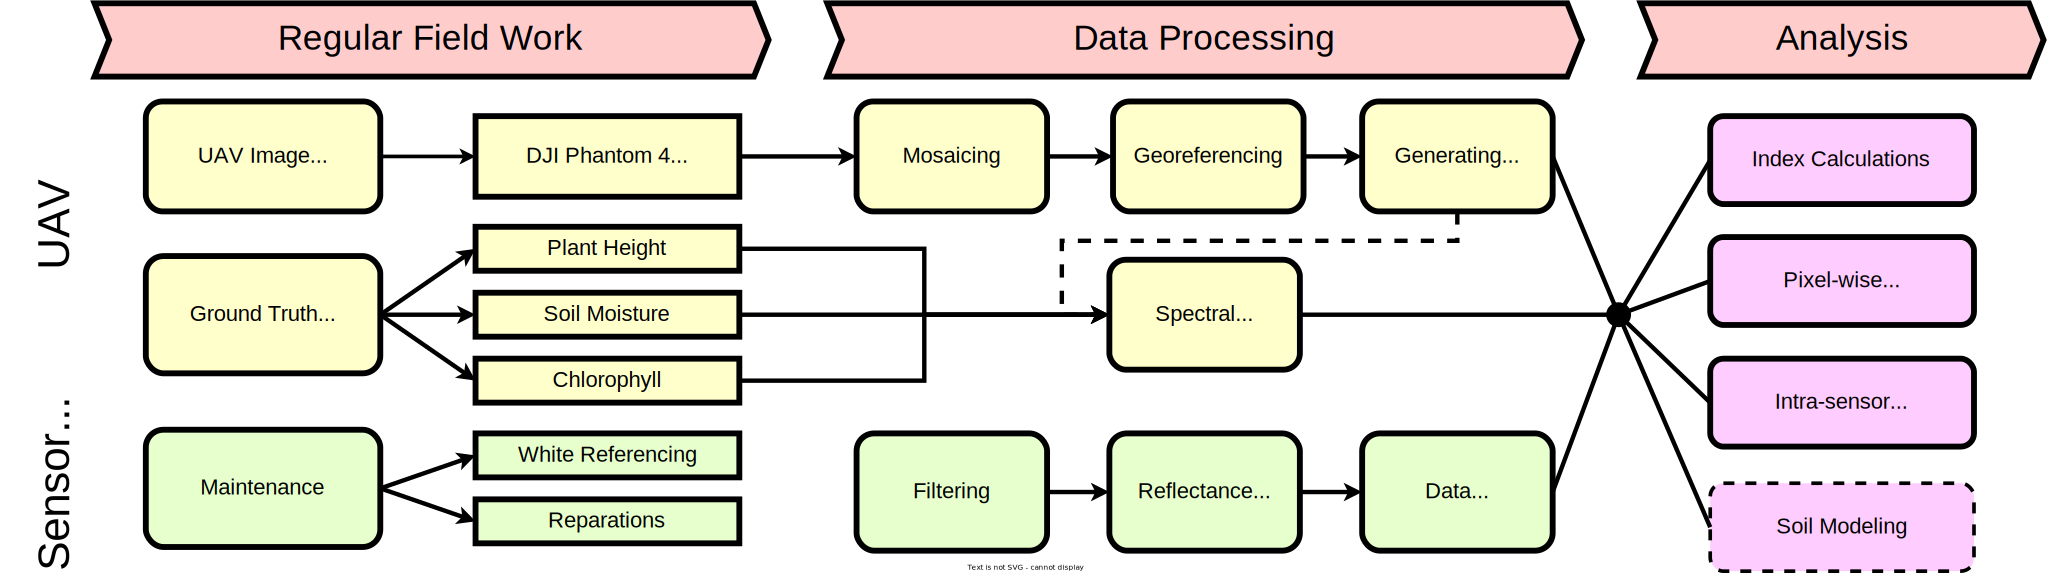
\includegraphics[width=.95\textwidth]{pics/workflow.png}
\end{minipage}
\end{block}

\vspace{-1.5cm}

\begin{minipage}[t][][t]{0.48\paperwidth}
\begin{block}{NDVI Comparison}
\begin{minipage}{0.16\paperwidth}

\resizebox{\textwidth}{!}{%
\begin{tikzpicture}[x=0.4cm,y=11cm]

\def\xmin{0} 
  \def\xmax{50} 
  \def\ymin{0} 
  \def\ymax{1.2} 


\draw[-] (\xmin,0) -- (\xmax,0) node[right] {Date}; 
   \draw[-] (\xmin,\ymin) -- (\xmin,\ymax) node[right] {NDVI, northern plot}; 

% tick marks and tick labels on axes 
        \foreach \x / \xlabel in {4/15.06, 19/30.06, 34/15.07, 49/30.07} 
                 \draw (\x,3pt) -- (\x,-6pt) 
                    node[anchor=north] {\xlabel}; 
        \foreach \y  in {0, 0.2,0.4, 0.6, 0.8, 1}
                 \draw (\xmin ,\y) -- (\xmin,\y) 
                         node[anchor=east]  {\y}; 
%sensor

\draw [-, line width=0.3mm, color=yellow!20] (7,0.00) -- (7,1.05);
\draw [-, line width=0.3mm, color=yellow!20] (21,0.00) -- (21,1.05);
\draw [-, line width=0.3mm, color=yellow!20] (35,0.00) -- (35,1.05);
\draw [-, line width=0.3mm, color=yellow!20] (46,0.00) -- (46,1.05);

 \foreach \Point in 
{( 4, 0.926656637742581),
(5, 0.903134735088708),
(6, 0.801206637136516),
(7, 0.898601993123537),
(8, 0.891902685186176),
(9, 0.92322453893563),
(10, 0.907423077209726),
(11, 0.908395397099545),
(12, 0.910476767050363),
(13, 0.887486871974987),
(14, 0.903887507506642),
(15, 0.883060477631159),
(16, 0.921937522732267),
(17, 0.898322205887492),
(21, 0.898034559367523),
(28, 0.839570698754296),
(29, 0.828395506441636),
(30, 0.798351495548504),
(31, 0.739635927837787),
(32, 0.762627066371609),
(33, 0.693522946102789), 
(34, 0.528736366859101),
(35, 0.522692245840823),
(36, 0.557176980218534),
(37, 0.494381341882956),
(38, 0.486923648746354),
(39, 0.42232583152893),
(40, 0.400074523186724),
(41, 0.363497442844717),
(42, 0.315494166501164),
(43, 0.285171372706176),
(44, 0.277311150144452),
(45, 0.233305365197851),
(46, 0.213418036771195)}{
    \node[circle,fill={rgb,255:red,204;green,255;blue,153},scale=0.5, minimum size=1pt] at \Point {};
}
%uav
 \foreach \Point in 
{( 7, 0.90304),
(21, 0.84619258473474),
(35, 0.640845070422535),
(46, 0.341840161182001)}{
    \node[circle,fill={rgb,255:red,255;green,153;blue,153},scale=0.5, minimum size=1pt] at \Point {};
}
%s2
 \foreach \Point in 
{( 7, 0.863918),
(27, 0.828830540180206),
(30, 0.720214664936065),
(37, 0.524619),
(42, 0.348075),
(45, 0.264281243085861)}{
    \node[circle,fill={rgb,255:red,153;green,204;blue,255},scale=0.5, minimum size=1pt] at \Point {};
}

\node at (14, 0.4) {$r_{UAV}$=0.99};
\node at (12.4, 0.3) {$r_{S2}$=0.99};
\end{tikzpicture}
}%

\vspace{0.5em}

\centering
\resizebox{\textwidth}{!}{%
\begin{tikzpicture}[x=0.4cm,y=11cm]

\def\xmin{0} 
  \def\xmax{50} 
  \def\ymin{0} 
  \def\ymax{1.2} 


\draw[-] (\xmin,0) -- (\xmax,0) node[right] {Date}; 
   \draw[-] (\xmin,\ymin) -- (\xmin,\ymax) node[right] {NDVI, southern plot}; 

% tick marks and tick labels on axes 
        \foreach \x / \xlabel in {4/15.06, 19/30.06, 34/15.07, 49/30.07} 
                 \draw (\x,3pt) -- (\x,-6pt) 
                    node[anchor=north] {\xlabel}; 
        \foreach \y  in {0, 0.2,0.4, 0.6, 0.8, 1}
                 \draw (\xmin ,\y) -- (\xmin,\y) 
                         node[anchor=east]  {\y}; 
                         
\draw [-, line width=0.3mm, color=yellow!20] (7,0.00) -- (7,1.05);
\draw [-, line width=0.3mm, color=yellow!20] (21,0.00) -- (21,1.05);
\draw [-, line width=0.3mm, color=yellow!20] (35,0.00) -- (35,1.05);
\draw [-, line width=0.3mm, color=yellow!20] (46,0.00) -- (46,1.05);                         
 
%sensor
 \foreach \Point in 
{( 4, 0.86387399081746),
(5, 0.804674140368141),
(6, 0.769277372437514),
(7, 0.840054218910279),
(21, 0.854852652222823),
(22, 0.806055171094352),
(23, 0.844115521403461),
(24, 0.833376049264745),
(25, 0.841278345567427),
(26, 0.800697559057925),
(27, 0.798639276973376),
(28, 0.797573576056134),
(29, 0.804663394831362),
(30, 0.748783490102206),
(31, 0.708901276396802),
(32, 0.727824006864923),
(33, 0.696247360512506),
(34, 0.694022772343952),
(35, 0.617069967860506),
(36, 0.411258791179303),
(37, 0.366306962192985),
(38, 0.437277842356267),
(39, 0.34889642727411),
(40, 0.364020245781453),
(41, 0.279749561285269),
(42, 0.229397781820312),
(43,0.259463932249297),
(44, 0.228083618403346),
(45, 0.260450068486249),
(46, 0.219469996042194)}{
    \node[circle,fill={rgb,255:red,204;green,255;blue,153},scale=0.5, minimum size=1pt] at \Point {};
}
%uav
 \foreach \Point in 
{( 7, 0.89675236828819),
(21, 0.834313271151559),
(35, 0.470858895705521),
(46, 0.255681502596437)}{
    \node[circle,fill={rgb,255:red,255;green,153;blue,153},scale=0.5, minimum size=1pt] at \Point {};
}
%s2
 \foreach \Point in 
{( 7, 0.802319),
(27, 0.790362417697906),
(30, 0.660020530223846),
(37, 0.494392),
(42, 0.328368),
(45, 0.264281243085861)}{
    \node[circle,fill={rgb,255:red,153;green,204;blue,255},scale=0.5, minimum size=1pt] at \Point {};
}


\node at (14, 0.4) {$r_{UAV}$=0.95};
\node at (12.4, 0.3) {$r_{S2}$=0.97};
\end{tikzpicture}
}%

\end{minipage}
\begin{minipage}{0.3\paperwidth}
\small{ Left: NDVI values for the three sensor systems for both observed plots. Below: Comparison of a subset of Sentinel 2 (top) and
UAV (bottom) NDVI time series with the calculated sensor NDVI values at the four marked dates}
\includegraphics[width = \textwidth]{maps/sentinel-p4.pdf}
\end{minipage}
\small{
\begin{itemize}
    \item All sensor systems can be used to map NDVI time series over the entire area
    \item NDVI values vary slightly, due to different spectral and spatial resolution, but show high correlation ($r=0.95$ - $r=0.99$)
\end{itemize}}
\vspace{0.21cm}
\end{block}
\end{minipage}
\hspace{4mm}
\begin{minipage}[t][][t]{0.48\paperwidth}
\begin{block}{Regression Results}
\begin{minipage}{0.17\paperwidth}
    \includegraphics[height=21cm]{pics/svr_20210603_moisture.png}
\end{minipage}
\begin{minipage}{0.14\paperwidth}
    \includegraphics[height=21cm]{pics/svr_20210618_height.png}
\end{minipage}
\begin{minipage}{0.15\paperwidth}
\small{
    \begin{itemize}
        \item Support Vector Regressions for soil moisture (left) and plant height (right) with grid searched parameters
        \item High degree of uncertainty in plant height regression: Correlation between height and spectral values seems low
        \item Promising initial results for soil moisture; experiment will be repeated with larger sample size
        %\item Results in mediocre $r^2$, regression for chlorophyll content impossible ($r^2$ around 0)
    \end{itemize}
    }
\end{minipage}
%\vspace{18cm}
\end{block}
\end{minipage}

\begin{block}{Conclusion \& Future Work}
\begin{minipage}{0.95\paperwidth}
\begin{minipage}{0.68\textwidth}
\small{
\begin{itemize}
    \item Each sensor has different advantages, as shown in the table on the right
    \item UAV data has proven itself useful to monitor side-specific small scale spatial differences and calculate plant characteristics with regression models based on ground truth measurements
    \item For further research, a larger ground truth sample size might be advantageous in order to reduce the influence of outliers
    \item Stationary sensors can be used to monitor differences at specific positions in a high temporal resolution and independent from weather conditions
    \item Further research should use a greater amount of sensors within the sensor network to show side-specific differences in a high temporal resolution
\end{itemize}
% - Stationäre Sens. für zeitlich hochaufgelöste Daten für detailliertes monitoring der Pflanzen Entwicklung, nicht auf den ganzen Schlag übertragbar,
% - UAV: räumlich hochaufgelöste Daten, die Hochrechnungen für ganzen Schlag zulassen, dafür hier die Stichprobe zu gering für präzise Aussagen
% - Satellit: Blick in die Vergangenheit möglich, großflächige Hochrechnung umsetzbar
}
\end{minipage}
\hspace{5cm}
\begin{minipage}{0.22\textwidth}
\centering
\fontsize{22pt}{24pt}\selectfont
\begin{table}[]
    \centering
    \begin{tabular}{rccc}
    \toprule
         & Sensor & UAV & S2 \\
     \midrule
         Historic data & && X \\
         Remote use & & & X\\
         High temporal resolution & X & & \\
         High spatial resolution & & X & \\
         Plant characteristics & X & X & X\\
         Side-specific monitoring & X & X & depends  \\
         & & & on size\\
         Weather independent & X & & \\
         Expandability of spectral bands & X & &\\
     \bottomrule   
    \end{tabular}
    \label{tab:my_label}
\end{table}
\end{minipage}

\end{minipage}
\end{block}

\begin{minipage}{0.65\paperwidth}
\begin{block}{References}
\begin{minipage}{0.95\textwidth}
\bibliographystyle{IEEEtranS}
{\tiny
\bibliography{IEEEabrv,references}}
\end{minipage}
\end{block}
\end{minipage}
\hspace{4mm}
\begin{minipage}{0.31\paperwidth}
\vspace{2cm}
\begin{minipage}[t][][t]{0.3\textwidth}
\centering
\vspace{8pt}
%\quad
%\tiny{CARPE MEMORIAM}
\qrcode[height=.75\textwidth]{https://sys.cs.uos.de/carpe_memoriam/}\\ 
\vspace*{10pt}
\tiny{CARPE MEMORIAM}
\vspace{1cm}
\end{minipage}
\begin{minipage}[t][][t]{0.35\textwidth}
\centering
\vspace{0pt}
%\tiny{test}
\includegraphics[width=0.99\textwidth]{pics/BMBF_gefoerdert_2017_en}
\tiny Funding reference: 01IS19045
\end{minipage}
\begin{minipage}[t][][t]{0.25\textwidth}
\centering
\vspace{22pt}
\includegraphics[width=0.99\textwidth]{pics/logo_dlr.png}
\tiny{Supervising institution}
\end{minipage}


\end{minipage}
\end{frame}                                            
\end{document}

